\chapter{Adapting to PCL}
Adapting pre-existing executables to PCL can be achieved in two ways, they are:
\begin{itemize}
\item \textbf{Imperative PCL}: The PCL language supports an imperative style grammar which allows component authors to use runtime libraries to run external executables. This portion of the PCL grammar is not \emph{Turing complete} since there are no looping constructs. This feature of PCL exists to quickly initialise pre-requisites of an external executable, run the executable, post-process a result, and return the result. If it turns out your component needs a more complex pre- and post-processing, or a component cannot be, or need not be an external exectuable, the second approach can be used.
\item \textbf{Python Wrapper}: A Python file, containing, six functions can be written that informs PCLc about the nature fo the component. Properties defined are: component's name, input and output port specifications, configuration and pre-processing configuration, and the component's computation. Since the computation of the component is described using Python, an arbitrarily complex component can be written.
\end{itemize}

Care must be taken when adapting your existing work to PCL pipelines. Threading issues and batch or on-line processing must be considered as the dynamics of your final pipeline may depend on it. Also, any state that may need to accumulate over the lifetime of a PCL component must be handled by the adaptor for your programs.

\section{Imperative PCL}
The imperative PCL language is a free-form language which allows the programmer to use arbitrary white-space to format your component definitions. Comments are a single line and should start with the \texttt{\#} and can appear at any point in a PCL file.
\begin{figure}[h!]
  \centering
    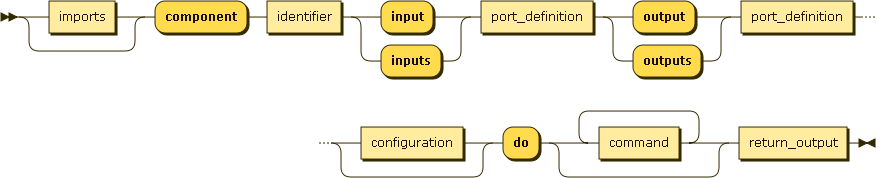
\includegraphics[scale=\DiagramScale,angle=90]{chapters/adapter/diagrams/component}
  \caption{Imperative PCL file syntax.}
  \label{fig:imperative-pcl-top-level}
\end{figure}
The top level syntax of a PCL file is shown in Figure \ref{fig:imperative-pcl-top-level}, and consists of the following sections:
\begin{itemize}
\item \textbf{Imports}: Imports can be optionally specified. The imports here are PCL runtime libraries. These are written in Python and are modules which contain functions. Imports must specify an alias and this is use to call the functions, e.g., \texttt{list.insert(...)}.
\item \textbf{Component}: This starts the component definition and provides the name. The component's name must be the same as the filename. E.g., a component in \texttt{fred.pcl} must be called \texttt{fred}.
\item \textbf{Inputs}: Defines the inputs of the component. This information is used to verify that the outputs of a previous component is compatible with another. Only \emph{one} input port can be defined.
\item \textbf{Outputs}: Defines the outputs of the component. This information is used to verify that the inputs of a subsequent component is compatible with another. Only \emph{one} output port can be defined.
\item \textbf{Configuration}: Optional configuration for the component. This is static data that shall be used to construct imported components used in this component. 
\item \textbf{Commands}: This portion is the component definition. It is a list of commands which are executed in order from top to bottom.
\end{itemize}

An example imperative PCL file can be seen in Figure \ref{fig:imperative-pcl-example}. This example can be found in the \texttt{parallel\_sleep} example in the PCL Git repository.
\begin{figure}[h!]
  \begin{verbatim}
import pcl.system.process as process
import pcl.util.list as list

component sleep
  input sleep_time
  output complete
  configuration sleep_command
  do
    cmd <- list.cons(@sleep_command, sleep_time)
    process.callAndCheck(cmd)

    return complete <- True
  \end{verbatim}
  \caption{Example imperative PCL file.}
  \label{fig:imperative-pcl-example}
\end{figure}

\subsection{Imports}
\begin{figure}[h!]
  \centering
    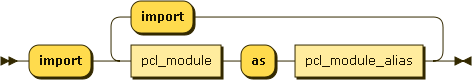
\includegraphics[scale=\DiagramScale]{chapters/adapter/diagrams/imports}
  \caption{\texttt{imports} : Importing PCL runtime functions.}
  \label{fig:imperative-pcl-imports}
\end{figure}
Imperative PCL files can use runtime library functions to import functionality. These runtime libraries are Python files which contain functions. The names of functions are the name of the function in PCL. Figure \ref{fig:imperative-pcl-imports} shows the syntax for importing. The environment variable \texttt{PCL\_IMPORT\_PATH} is a colon separated list of directories from which a search shall take place for the PCL runtime libraries. If this environment variable is not set then the current working directory is used as a starting point for the component search.

Each imported component must specify an alias. This is the name by which this component shall be referred to in this PCL file. E.g., \texttt{import pcl.util.list as list} shall import a PCL runtime library called \texttt{list} from the package \texttt{pcl.util} and shall be refereed to as, i.e. has the alias, \texttt{list}.

Figure \ref{fig:imperative-pcl-import-non-terminals} shows how the non-terminals expand in the import syntax.
\begin{figure}[h!]
  \centering
  \begin{subfigure}[b]{0.4\textwidth}
    
\includegraphics[scale=\DiagramScale]{chapters/adapter/diagrams/pcl_module}
    \caption{\texttt{pcl\_module} expansion}
  \end{subfigure}
  ~
  \begin{subfigure}[b]{0.4\textwidth}
    
\includegraphics[scale=\DiagramScale]{chapters/adapter/diagrams/pcl_module_alias}
    \caption{\texttt{pcl\_module\_alias} expansion}
  \end{subfigure}
  \caption{\texttt{pcl\_module} \& \texttt{pcl\_module\_alias} : Imperative import PCL non-terminals.}
  \label{fig:imperative-pcl-import-non-terminals}
\end{figure}

\subsection{Port Definition}
\begin{figure}[h!]
  \centering
    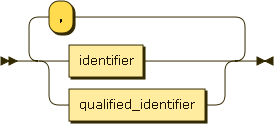
\includegraphics[scale=\DiagramScale]{chapters/adapter/diagrams/port_definition}
  \caption{\texttt{port\_definition} : Imperative PCL port definition.}
  \label{fig:imperative-pcl-port-def}
\end{figure}
A port definition informs the PCL compiler about the nature of a component's input or an output. Components defined with imperative PCL can only have one input and one output port. Figure \ref{fig:pcl-port-def} shows the syntax for this grammatical construct.

Again, ports carry one or more \emph{signals}. A signal is a piece of data that flows through ports and has a unique name to that port, and can be fully qualified. The signal names, for a port, are declared in a port definition. Signal names are read-only.

\subsection{Configuration}
\begin{figure}[h!]
  \centering
    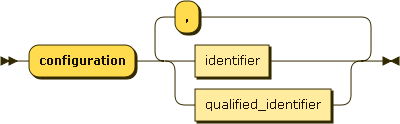
\includegraphics[scale=\DiagramScale]{chapters/adapter/diagrams/configuration}
  \caption{\texttt{configuration} : Imperative PCL configuration.}
  \label{fig:imperative-pcl-config}
\end{figure}
A component's configuration is static and read-only data. Configuration data is named using identifiers, which can be fully qualified. Figure \ref{fig:imperative-pcl-config} shows the configuration syntax. Configuration identifiers may be used at any point where a variable, or input signal name can be used, e.g., and \emph{if} command, or function call. In imperative PCL zero or more configuration identifiers can be declared.

\subsection{Commands}
The command syntax is shown in Figure \ref{fig:imperative-pcl-command}. Each command yields a value which can, optionally, be assign to a write-once ``variable''. 
\begin{figure}[h!]
  \centering
    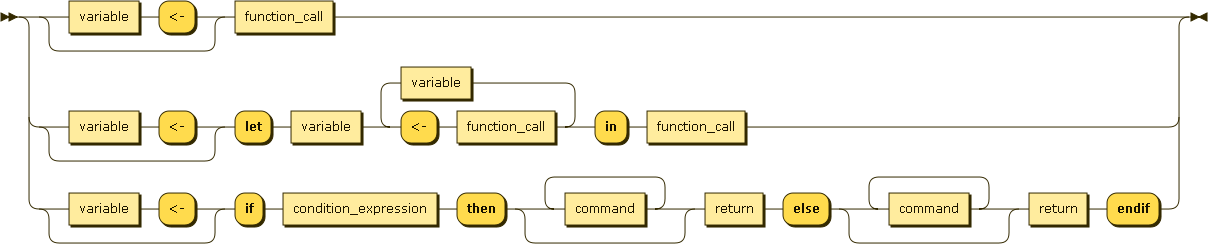
\includegraphics[scale=0.45,angle=90]{chapters/adapter/diagrams/command}
  \caption{\texttt{command} : Imperative PCL commmands.}
  \label{fig:imperative-pcl-command}
\end{figure}

\subsubsection{Function Calls}
The PCL runtime functions can be used in an imperative PCL component using the following syntax shown in Figure \ref{fig:imperative-pcl-function-call}.
\begin{figure}[h!]
  \centering
    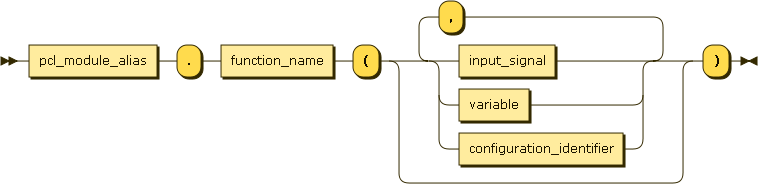
\includegraphics[scale=0.45]{chapters/adapter/diagrams/function_call}
  \caption{\texttt{function\_call} : Imperative PCL function call.}
  \label{fig:imperative-pcl-function-call}
\end{figure}
Functions are called using the import alias, assigned in the import statement, and the function name, e.g., \texttt{list.insert(...)}. A function call's arguments can be any one of an input signal, variable or configuration values, e.g., the call \texttt{list.cons(filename, @working.directory, extension)} constructs a list using the input signal \texttt{filename}, the configuration \texttt{working.directory}, and a variable \texttt{extension}. This list could be assigned to a variable using the following \texttt{pathname <- list.cons(filename, @working.directory, extension)}. The variable \texttt{pathname} is readable in all scopes below the current scope.

Runtime functions can be written by users and should be in Python modules, i.e., a directory containing the file \texttt{\_\_init\_\_.py}. These files should contain only functions, e.g., see Figure \ref{fig:imperative-pcl-runtime-library} for an example of the runtime library \texttt{pcl.util.string}.
\begin{figure}[h!]
  \begin{verbatim}
split = lambda s, ss: s.__str__().split(ss)

join = lambda l, s: s.join([str(e) for e in l])

lower = lambda s: s.__str__().lower()

upper = lambda s: s.__str__().upper()
  \end{verbatim}
  \caption{\texttt{string.py}: An example of a runtime library.}
  \label{fig:imperative-pcl-runtime-library}
\end{figure}
In order for PCLc to ``see'' these library modules the \texttt{PCL\_IMPORT\_PATH} environment variable must specify the directory in which these Python modules can be found.

Figure \ref{fig:imperative-pcl-function-call-non-terminals} shows how the non-terminals expand in a function call.
\begin{figure}[h!]
  \centering
  \begin{subfigure}[b]{0.4\textwidth}
    
\includegraphics[scale=\DiagramScale]{chapters/adapter/diagrams/function_name}
    \caption{\texttt{function\_name} expansion}
  \end{subfigure}
  ~
  \begin{subfigure}[b]{0.4\textwidth}
    
\includegraphics[scale=\DiagramScale]{chapters/adapter/diagrams/input_signal}
    \caption{\texttt{input\_signal} expansion}
  \end{subfigure}

  \begin{subfigure}[b]{0.4\textwidth}
    
\includegraphics[scale=\DiagramScale]{chapters/adapter/diagrams/variable}
    \caption{\texttt{variable} expansion}
  \end{subfigure}
  ~
  \begin{subfigure}[b]{0.4\textwidth}
    
\includegraphics[scale=\DiagramScale]{chapters/adapter/diagrams/configuration_identifier}
    \caption{\texttt{configuration\_identifier} expansion}
  \end{subfigure}
  \caption{\texttt{function\_name} \& \texttt{input\_signal} \& \texttt{variable} \& \texttt{configuration\_identifier}: Imperative PCL function call non-terminals.}
  \label{fig:imperative-pcl-function-call-non-terminals}
\end{figure}

\subsubsection{Let Bindings}
Let bindings allow variables to be scoped so that only the function call in the \emph{in} clause has access to them. For example, Figure \ref{fig:imperative-pcl-let-binding-example} shows a let binding which builds a new pathname for a supplied filename and working directory. Notice all input signals and configuration are accessable inside the let binding. Moreover, any assigned variables before the let binding would be accessable. All variables assigned inside the let binding are only accessable inside of the let binding. Finally, the value of the \texttt{path.join()} function is assigned to the \texttt{pathname} variable.
\begin{figure}[h!]
  \begin{verbatim}
import pcl.os.path as path
import pcl.util.list as list
import pcl.util.string as string

component pathname_creator
  input filename
  output filename.new
  configuration working.directory
  do
    pathname <- let
                  basename <- path.basename(filename)
                  pieces <- path.splitext(basename)
                  base <- list.index(pieces, 0)
                  ext <- list.index(pieces, 1)
                  bits <- list.cons(base, "new", ext)
                  new_basename <- string.join(bits, ".")
                in
                  path.join(@working.directory, new_basename)

    return filename.new <- pathname
  \end{verbatim}
  \caption{Let binding example}
  \label{fig:imperative-pcl-let-binding-example}
\end{figure}

\subsubsection{If Commands}
\emph{If} commands in imperative PCL are similar to ternary operators available in many computing languages. However, \emph{If} commands in PCL are more powerful and allow other commands to be executed from within the \texttt{then} and \texttt{else} blocks. Since all commands in imperative PCL have a value both the \texttt{then} and \texttt{else} blocks must be specified, and use the \texttt{return} keyword to create a value for when the condition is true or false. If no value is to be generated then the special \texttt{return ()} statement can be used. Otherwise, the value of a variable can be made available for assignment, e.g., Figure \ref{fig:imperative-pcl-if-example} shows an example of how to evaluate a value and not a value.
\begin{figure}[h!]
  \begin{verbatim}
import pcl.os.path as path
import pcl.util.list as list
import pcl.util.string as string

component pathname_creator
  input filename
  output filename.new
  configuration working.directory
  do
    pathname <- if then

    else
  
    endif

    return filename.new <- pathname
  \end{verbatim}
  \caption{\emph{If} example}
  \label{fig:imperative-pcl-if-example}
\end{figure}

\section{Python Wrapper}
The Python wrappers for your programs can inhabit the same hierarchical package structure as your PCL hierarchy. This is because the PCL hierarchy mirrors the Python one\footnote{This is the reason why \texttt{\_\_init\_\_.py} files must be manually placed in directories in your PCL heirarchy which have no PCL files.}.

Six functions are required in your Python wrapper, they are:
\begin{itemize}
\item \texttt{get\_name()}: Returns an object representing the name of the component. The \texttt{\_\_str\_\_()} function should be implemented to return a meaninful name. E.g.,
\begin{verbatim}
def get_name():
  return 'tokenisation'
\end{verbatim}
\item \texttt{get\_inputs()}: Returns the inputs of the component. Components should only be defined with one input port, which is defined by returning a single list of input port signal names. E.g.,
\begin{verbatim}
def get_inputs():
  return ['port.in.a', 'port.in.b']
\end{verbatim}
\item \texttt{get\_outputs()} - Returns the outputs of the component. Components should only be defined with one output port, which is defined by returning a single list of output port signal names. E.g.,
\begin{verbatim}
def get_outputs():
  return ['port.out.a', 'port.out.b', 'port.out.c']
\end{verbatim}
\item \texttt{get\_configuration()}: Returns a list of names that represent the static data that shall be used to construct the component. E.g.,
\begin{verbatim}
def get_configuration():
  return ['buffer.file', 'buffer.size']
\end{verbatim}
\item \texttt{configure(args)}: This function is the component designer's chance to preprocess configuration injected at runtime. The \texttt{args} parameter is a dictionary that contains all the configuration provided to the entire pipeline. This function is to filter out, and optionally preprocess, the configuration used by this component. This function shall return an object containing configuration necessary to construct this component. E.g. this example returns a dictionary of configuration,
\begin{verbatim}
import os
def configure(args):
  buffer_file = os.path.abspath(args['buffer.file'])
  return {'buffer.dir' : os.path.dirname(buffer_file),
          'buffer.file' : os.path.basename(buffer_file),
          'buffer.size' : args['buffer.size']}
\end{verbatim}
\item \texttt{initialise(config)}: This function is where the component designer defines the component's computation. The function receives the object returned from the \texttt{configure()} function and must return a function that takes two parameters, an input object, and a state object. The input object, \texttt{a} in the example below, is a dictionary that is received from the previous component in the pipeline. The keys of this dictionary are the signal names from the previous component's output port. The state object, \texttt{s} in the example below, is a dictionary containing the configuration for the component. The keys of the configuration dictionary are defined by the \texttt{get\_configuration()} function. The returned function should be used to define the component's computation. E.g.,
\begin{verbatim}
import subprocess
def initialise(config):
  def sleep_function(a, s):
    proc = subprocess.Popen([config['sleep_command'],
                             str(a['sleep_time'])])
    proc.communicate()
    return {'complete' : True}

  return sleep_function
\end{verbatim}
The function returned by \texttt{initialise()} is executed in the thread pool used by the runtime (see Chapter \ref{chap:runtime}). It is implementation defined as to whether this function blocks, waiting for a computation to complete, or not.
\end{itemize}

An example of a complete Python wrapper file is shown in Figure \ref{fig:python-wrapper}.
\begin{figure}[h!]
\begin{verbatim}
import subprocess

def get_name():
  return "sleep"

def get_inputs():
  return ['sleep_time']

def get_outputs():
  return ['complete']

def get_configuration():
  return ['sleep_command']

def configure(args):
  return {'sleep_command' : args['sleep_command']}

def initialise(config):
  def sleep_function(a, s):
    proc = subprocess.Popen([config['sleep_command'],
                             str(a['sleep_time'])])
    proc.communicate()
    return {'complete' : True}

  return sleep_function
\end{verbatim}
\caption{\texttt{sleep.py}: An example Python wrapper for PCL.}
\label{fig:python-wrapper}
\end{figure}
This wrapper is the Python implementation of the imperative PCL \texttt{sleep} component shown in Figure \ref{fig:imperative-pcl-example}.
